\documentclass[a4paper, 12pt]{article}
\usepackage[brazil]{babel}  	  % nomes de seções e títulos em Pt-BR
\usepackage[utf8]{inputenc} 	  % codificação de texto compatível com Pt-BR
\usepackage[T1]{fontenc}
\usepackage{physics, mathtools}
\usepackage{amsmath, amssymb, amsthm, amsfonts} % pacotes da AMS para ambientes matemáticos
\usepackage[final]{microtype} %melhora a tipografia do texto.
\usepackage{hyperref} % cria hyperlinks para equações, teoremas, etc
% \usepackage{showlabels} %Mostra os nomes dos labels.
\usepackage{graphicx, color}      % pacote para a inclusao de figuras em jpg, pdf, png e textos coloridos
\usepackage{epstopdf, epsfig}	  % pacote para a conversao de eps para pdf
\usepackage{latexsym}
\usepackage{subfigure, wrapfig}
\usepackage{indentfirst}
\usepackage[table]{xcolor}
\usepackage{tabularx, scalefnt}
\usepackage{multicol, multirow}
\usepackage{calc}
\usepackage{ifthen}
\usepackage{pdfpages}
\usepackage{fancyhdr}
\usepackage{circuitikz}
\usepackage{url}
\usepackage{lastpage}
\usepackage[top=3cm, left=3cm, right=2cm, bottom=2cm]{geometry}

\begin{document}

% CRIANDO A CAPA DO RELATÓRIO DE FÍSICA EXPERIMENTAL

\begin{center}
	
\includegraphics[scale=0.08]{./pictures/brasao.png}\\
	{\footnotesize {\bf MINISTÉRIO DA EDUCAÇÃO\\
		SECRETARIA DE EDUCAÇÃO PROFISSIONAL, CIENTÍFICA E TECNOLÓGICA\\
		INSTITUTO FEDERAL DE EDUCAÇÃO, CIÊNCIA E TECNOLOGIA
		CATARINENSE\\
		\textit{CAMPUS} SÃO BENTO DO SUL\\
		BACHARELADO EM ENGENHARIA DE COMPUTAÇÃO}}

	\vspace{5cm}
	\textbf{DETERMINAÇÃO DA ACELERAÇÃO DA GRAVIDADE ATRAVÉS DO PLANO INCLINADO DE GALILEU GALILEI}

	\vspace{3cm}
	\begin{tabular}{|l|l|}
		\hline
		{\bf Disciplina:} Física Experimental I        & {\bf Turma:} ECO2025/
		2                                                                             \\ \hline
		{\bf Professor:} Genilson Carvalho             & genilson.carvalho@ifc.edu.br \\ \hline
		{\bf Responsável:} Nelson Dias Ponciano Scarin & nelsonscarin34@gmail.com     \\ \hline
		Johnnathan Victor Gonçalves Sabbá              & victorsabba@gmail.com        \\ \hline
		Nome e Sobrenome                               & e-mail                       \\ \hline
		Nome e Sobrenome                               & e-mail                       \\ \hline
	\end{tabular}

	\vspace{7cm}
	São Bento do Sul - SC\\
	\today
\end{center}
\newpage

% INICIANDO O RELATÓRIO	
\twocolumn[
	\begin{center}
		\textbf{DETERMINAÇÃO DA ACELERAÇÃO DA GRAVIDADE ATRAVÉS DO PLANO INCLINADO DE GALILEU}
	\end{center}
	\vspace{0.5cm}
	\begin{center}
		\begin{minipage}{16.0cm}
			\textbf{RESUMO.} {\it Este relatório apresenta a determinação experimental da aceleração da gravidade utilizando o plano inclinado de Galileu. O experimento utilizou rampa de fio de nylon com ângulos de 30° e 60°, objetos metálicos e cronômetro digital. Foram realizadas 10 medições para cada ângulo, obtendo tempos médios de 0,701 s (30°) e 0,410 s (60°). Os valores calculados de g foram 8,14 m/s² e 7,97 m/s², resultando em valor médio de 8,06 m/s² com erro relativo de 17,9\% em relação ao valor teórico.}\\
			\textbf{Palavras-chave:} Plano inclinado; Aceleração da gravidade; Galileu Galilei; Física experimental.
		\end{minipage}
	\end{center}]

\section{Introdução}\label{intro}
Ao longo da história da fisica, muitos experimentos foram realizados para determinar o valor da aceleração da gravidade, sendo os mais notáveis aqueles realizados por Galileu Galilei \cite{Bezerra}. Galileu foi um dos primeiros a utilizar o método científico para investigar a natureza, e seus experimentos com planos inclinados foram essencias para a determinação fundamental no estudo do Movimento Uniformemente acelerado/variado (MUV) \cite{Brito}.

Na realização e observação de tal experimento Galileu, como descrito em \cite{Galilei}, Galileu constatou que o tempo que o objeto levava para percorrer o comprimento do plano era constante e que a massa do objeto não influenciava na aceleração.

\begin{figure}[!htpb]
	\centering
	\caption{Plano inclinado.}
	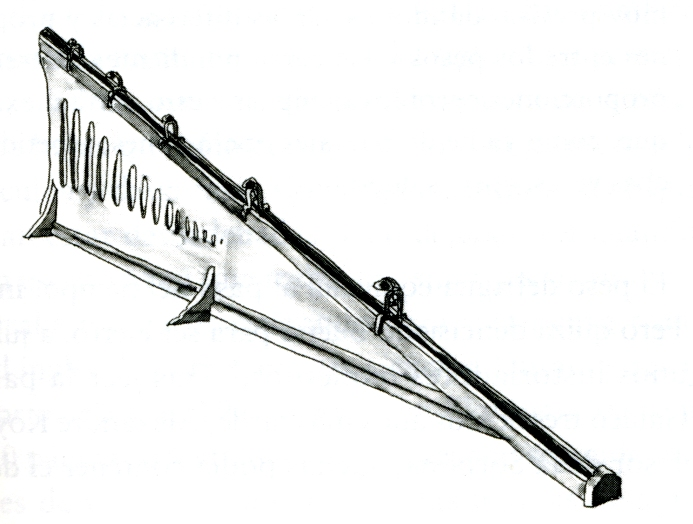
\includegraphics[scale=0.25]{./pictures/planoInclinado.png}
	Fonte: Galileu, Duas novas ciências, pp. 140-141, trad. Mariconda. P. R. Mariconda \& J. Vasconcelos, Galileu e a nova física, p. 44.
\end{figure}

A demonstraçao de tal experiemento, o qual já foi amplamente validado e estudado ao longo da historia, ainda é de extrema importância principalmente no contexto educacional \cite{Silva2023}, pois nos permite observar e compreender os principios fundamentais da fisica clássica além do papél, mas apartir de uma abordagem pratica experimental, auxiliando na fixação do conhecimento e na contrução do raciocinio anlitico e científico.

O objetivo deste relatório é descrever a metodologia utilizada para realizar o experimento de Galileu com um plano inclinado, apresentar os resultados obtidos e discutir as conclusões que podem ser tiradas a partir desses resultados. Através deste experimento, buscamos não apenas determinar o valor da aceleração da gravidade, mas também compreender melhor os princípios do movimento uniformemente acelerado e a influência da inclinação do plano nesse movimento.


\section{Metodologia}
Nesta seção são descritos os procedimentos empregados para efetuar as medidas e são descritas as montagens experimentais utilizadas.

\subsection{Materiais Utilizados}
\begin{itemize}
	\item \textbf{Rampa:} fio de nylon com comprimento de 1,0 m
	\item \textbf{Objetos em queda:} porcas e braçadeiras metálicas
	\item \textbf{Cronômetro:} digital com precisão de 0,01 s
	\item \textbf{Trena:} métrica com precisão de 1 mm
	\item \textbf{Transferidor:} para medição dos ângulos de inclinação
\end{itemize}

\subsection{Procedimento Experimental}
O experimento foi conduzido seguindo as etapas:
\begin{enumerate}
	\item Montagem do plano inclinado utilizando fio de nylon \newline como rampa
	\item Ajuste da inclinação para ângulos de 30° e 60°
	\item Medição das distâncias percorridas: 1,0 m para 30° e 0,58 m para 60°
	\item Realização de 10 medições de tempo para cada configuração angular
	\item Registro sistemático dos dados obtidos
\end{enumerate}

O tempo foi cronometrado desde o momento da liberação do objeto até sua chegada ao final da rampa. Para minimizar erros sistemáticos, as medições foram repetidas 10 vezes para cada ângulo, permitindo cálculo da média e análise da dispersão dos dados.

\section{Resultados e Discussões}
Esta seção apresenta os dados obtidos experimentalmente e sua análise comparativa com os valores teóricos esperados.

\subsection{Dados Experimentais}

\begin{table}[!htpb]
	\centering
	\caption{Tempos medidos para plano inclinado a 30°}
	\small
	\begin{tabular}{|c|c||c|c|}
		\hline
		\textbf{Tentativa} & \textbf{Tempo (s)} & \textbf{Tentativa} & \textbf{Tempo (s)} \\ \hline
		1                  & 0,68               & 6                  & 0,69               \\ \hline
		2                  & 0,71               & 7                  & 0,73               \\ \hline
		3                  & 0,69               & 8                  & 0,71               \\ \hline
		4                  & 0,72               & 9                  & 0,70               \\ \hline
		5                  & 0,70               & 10                 & 0,68               \\ \hline
		\multicolumn{4}{|c|}{\textbf{Tempo médio: 0,701 s}}                               \\ \hline
	\end{tabular}
\end{table}

\begin{table}[!htpb]
	\centering
	\caption{Tempos medidos para plano inclinado a 60°}
	\small
	\begin{tabular}{|c|c||c|c|}
		\hline
		\textbf{Tentativa} & \textbf{Tempo (s)} & \textbf{Tentativa} & \textbf{Tempo (s)} \\ \hline
		1                  & 0,41               & 6                  & 0,41               \\ \hline
		2                  & 0,40               & 7                  & 0,40               \\ \hline
		3                  & 0,42               & 8                  & 0,42               \\ \hline
		4                  & 0,39               & 9                  & 0,41               \\ \hline
		5                  & 0,43               & 10                 & 0,40               \\ \hline
		\multicolumn{4}{|c|}{\textbf{Tempo médio: 0,410 s}}                               \\ \hline
	\end{tabular}
\end{table}

\subsection{Cálculos e Análise}

Utilizando a equação fundamental do movimento uniformemente acelerado ($s = \frac{1}{2}at^2$) e a relação $a = g \sin(\theta)$, obtém-se:

$$g = \frac{2s}{t^2 \sin(\theta)}$$

\textbf{Para 30°:}
$$a_{30} = \frac{2 \times 1,0}{(0,701)^2} = 4,07 \text{ m/s}^2$$
$$g_{30} = \frac{4,07}{\sin(30)} = \frac{4,07}{0,5} = 8,14 \text{ m/s}^2$$

\textbf{Para 60°:}
$$a_{60} = \frac{2 \times 0,58}{(0,410)^2} = 6,90 \text{ m/s}^2$$
$$g_{60} = \frac{6,90}{\sin(60)} = \frac{6,90}{0,866} = 7,97 \text{ m/s}^2$$

\subsection{Discussão dos Resultados}

O valor médio obtido foi $g = 8,06$ m/s², que apresenta um erro relativo de 17,9\% em relação ao valor teórico (9,81 m/s²). Este erro pode ser atribuído a fatores como:
\begin{itemize}
	\item Tempo de reação humano na cronometragem
	\item Atrito entre o objeto e a superfície da rampa
	\item Imprecisões na medição dos ângulos
	\item Oscilações do objeto durante o movimento
\end{itemize}

Os resultados são consistentes entre os dois ângulos testados, validando a metodologia empregada.
Um outro ponto que gostariamos de enfatizar é que a velocidade final em ambos os casos são bem semelhantes, o que é esperado, ja que partindo do reposouo o objeto sofre uma aceleraçao constante, send o a altura do plano o unico fator relevante para a determinaçao da velocidade final, o que é confirmado pelos resultados obtidos.
Todavia devido a imprecisões em nossa na nossa obtencão de dados os valores obtidos da velocidade final final não identicos, mas ainda ssim muito proximos, o que reforça a validade do experimento.
Nas figuras \ref{fig:velocidade_tempo_obtido} e \ref{fig:velocidade_tempo_esperado} podemos observar os gráficos da velocidade em função do tempo obtido experimentalmente e o esperado, embasado nos valores teóricos.

\begin{figure}[!htpb]
	\centering
	\caption{Velocidade em função do tempo obtido.}
	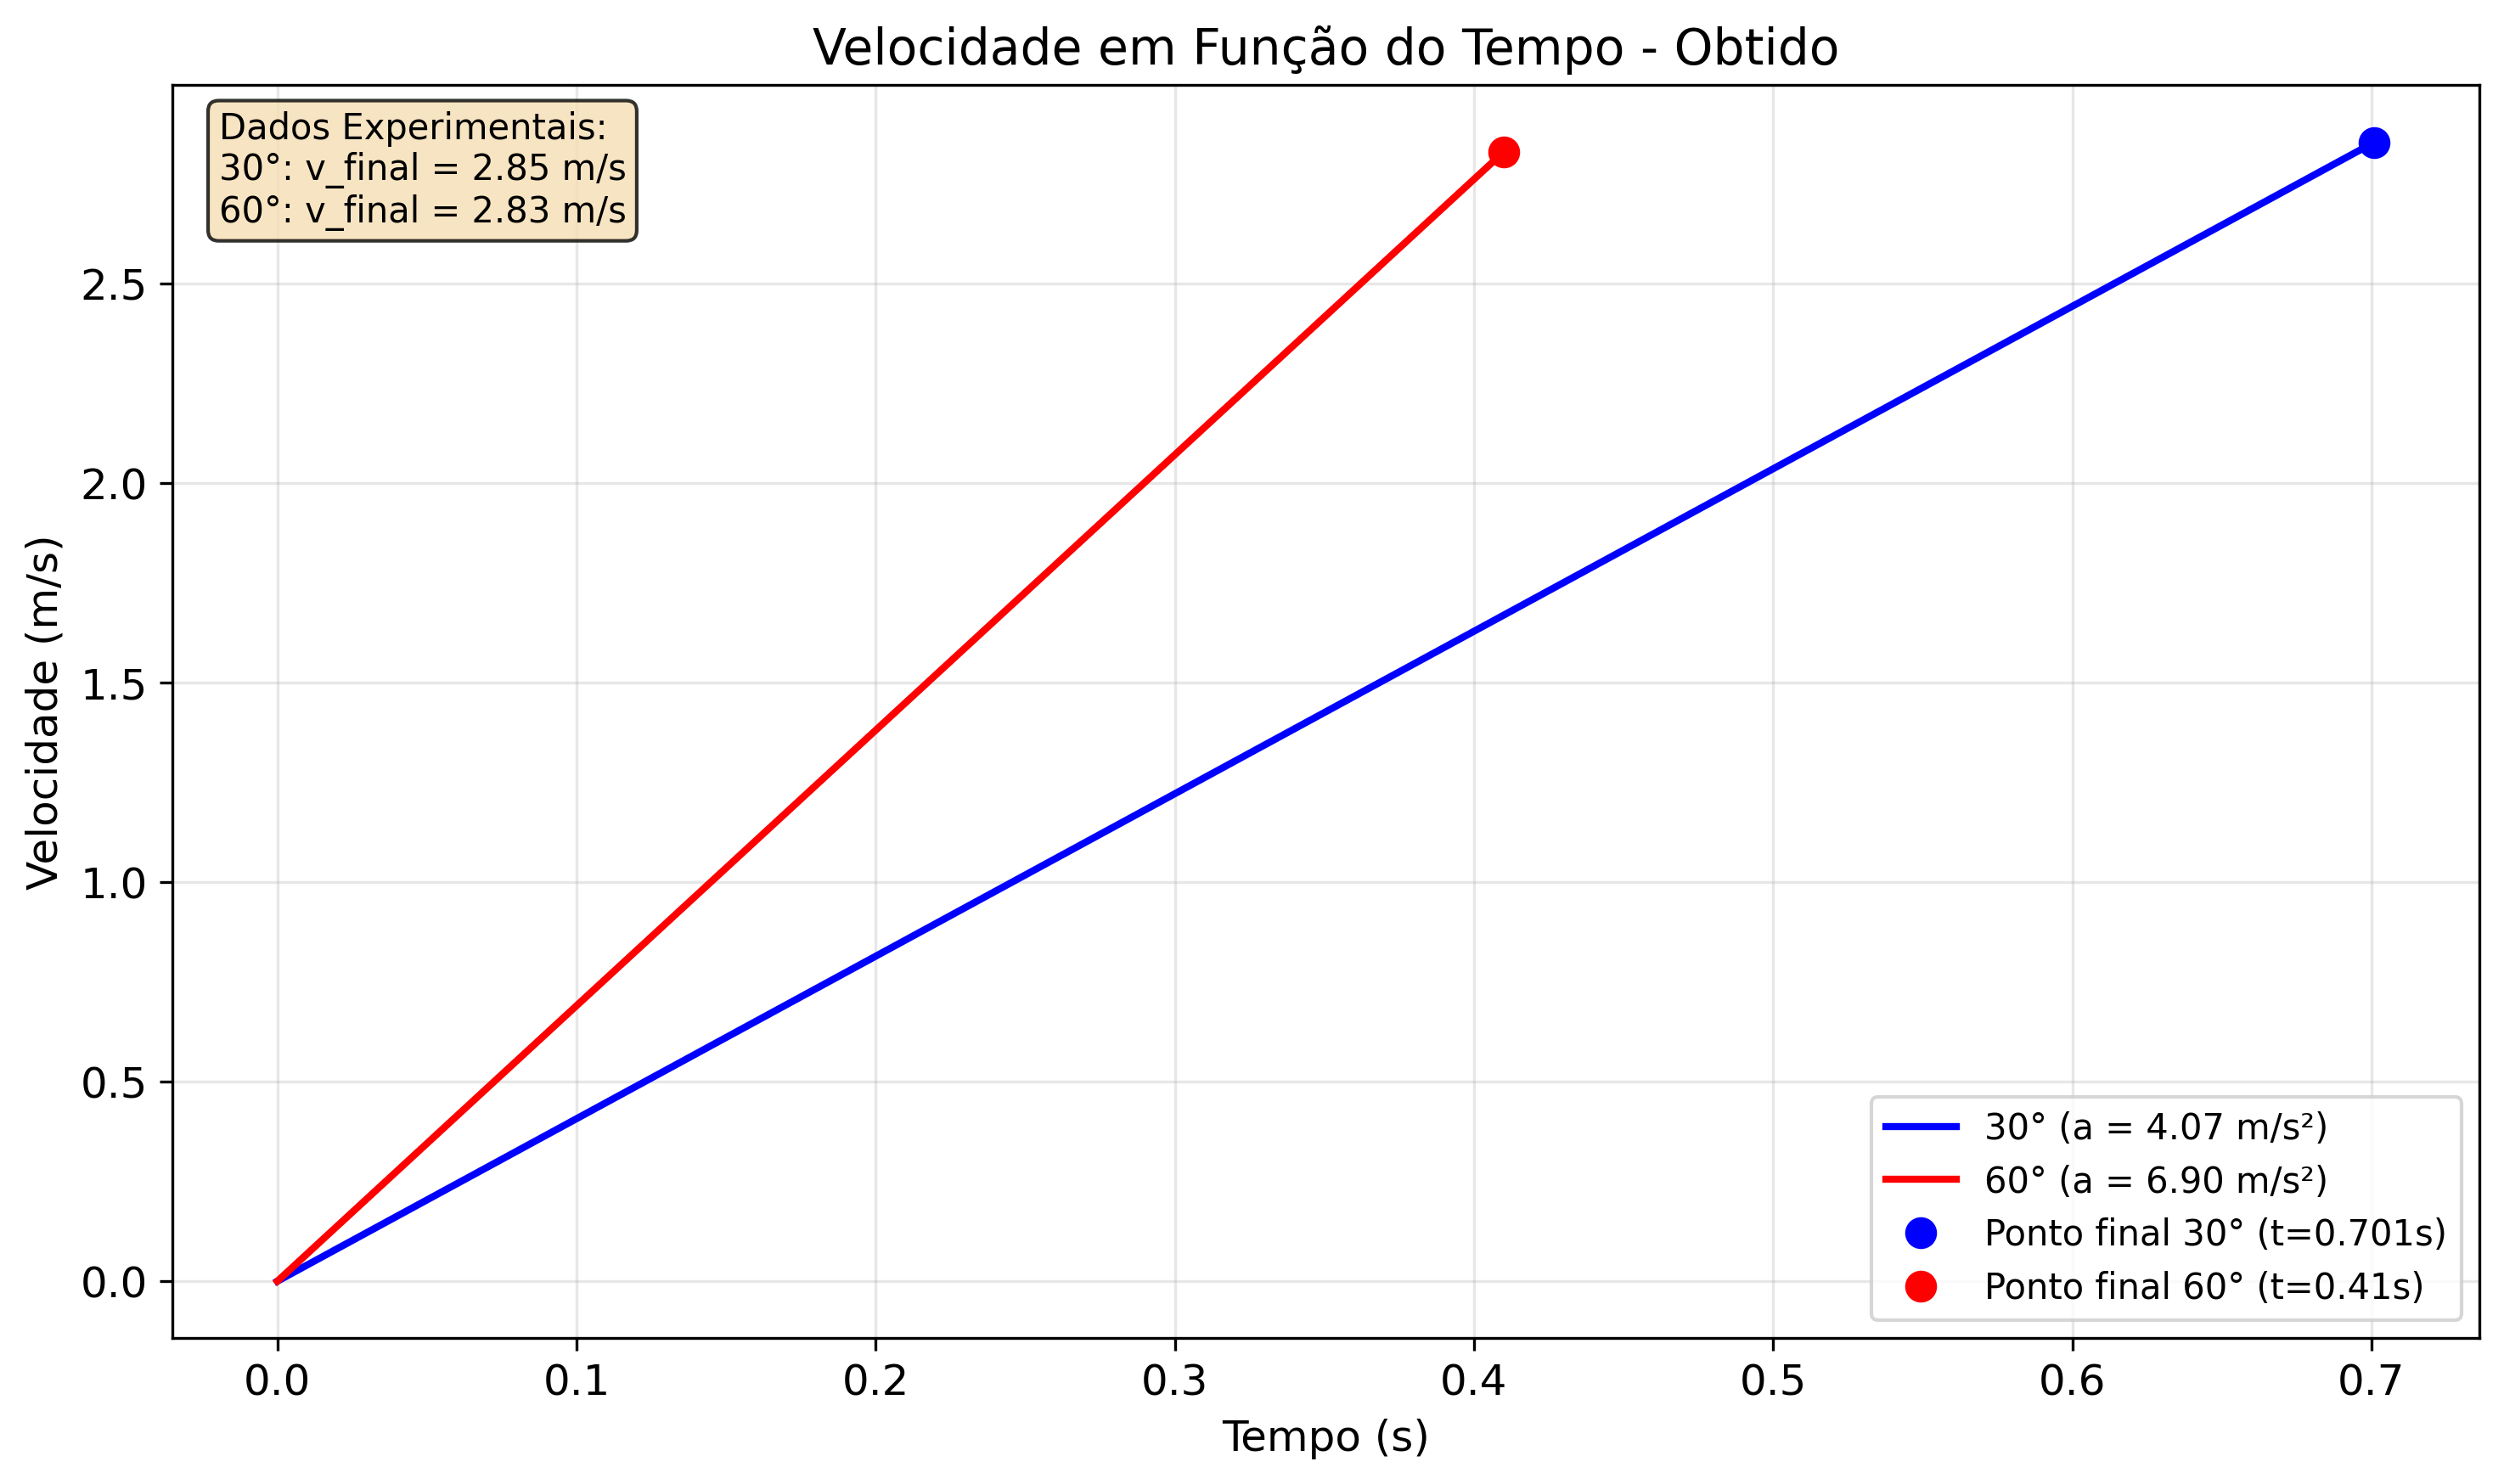
\includegraphics[scale=0.3]{./pictures/velocidade_tempo_obtido.png}
	\label{fig:velocidade_tempo_obtido}
	Fonte: Elaborado pelos autores utilizando Python (Matplotlib e NumPy).
\end{figure}

\begin{figure}[!htpb]
	\centering
	\caption{Velocidade em função do tempo esperado.}
	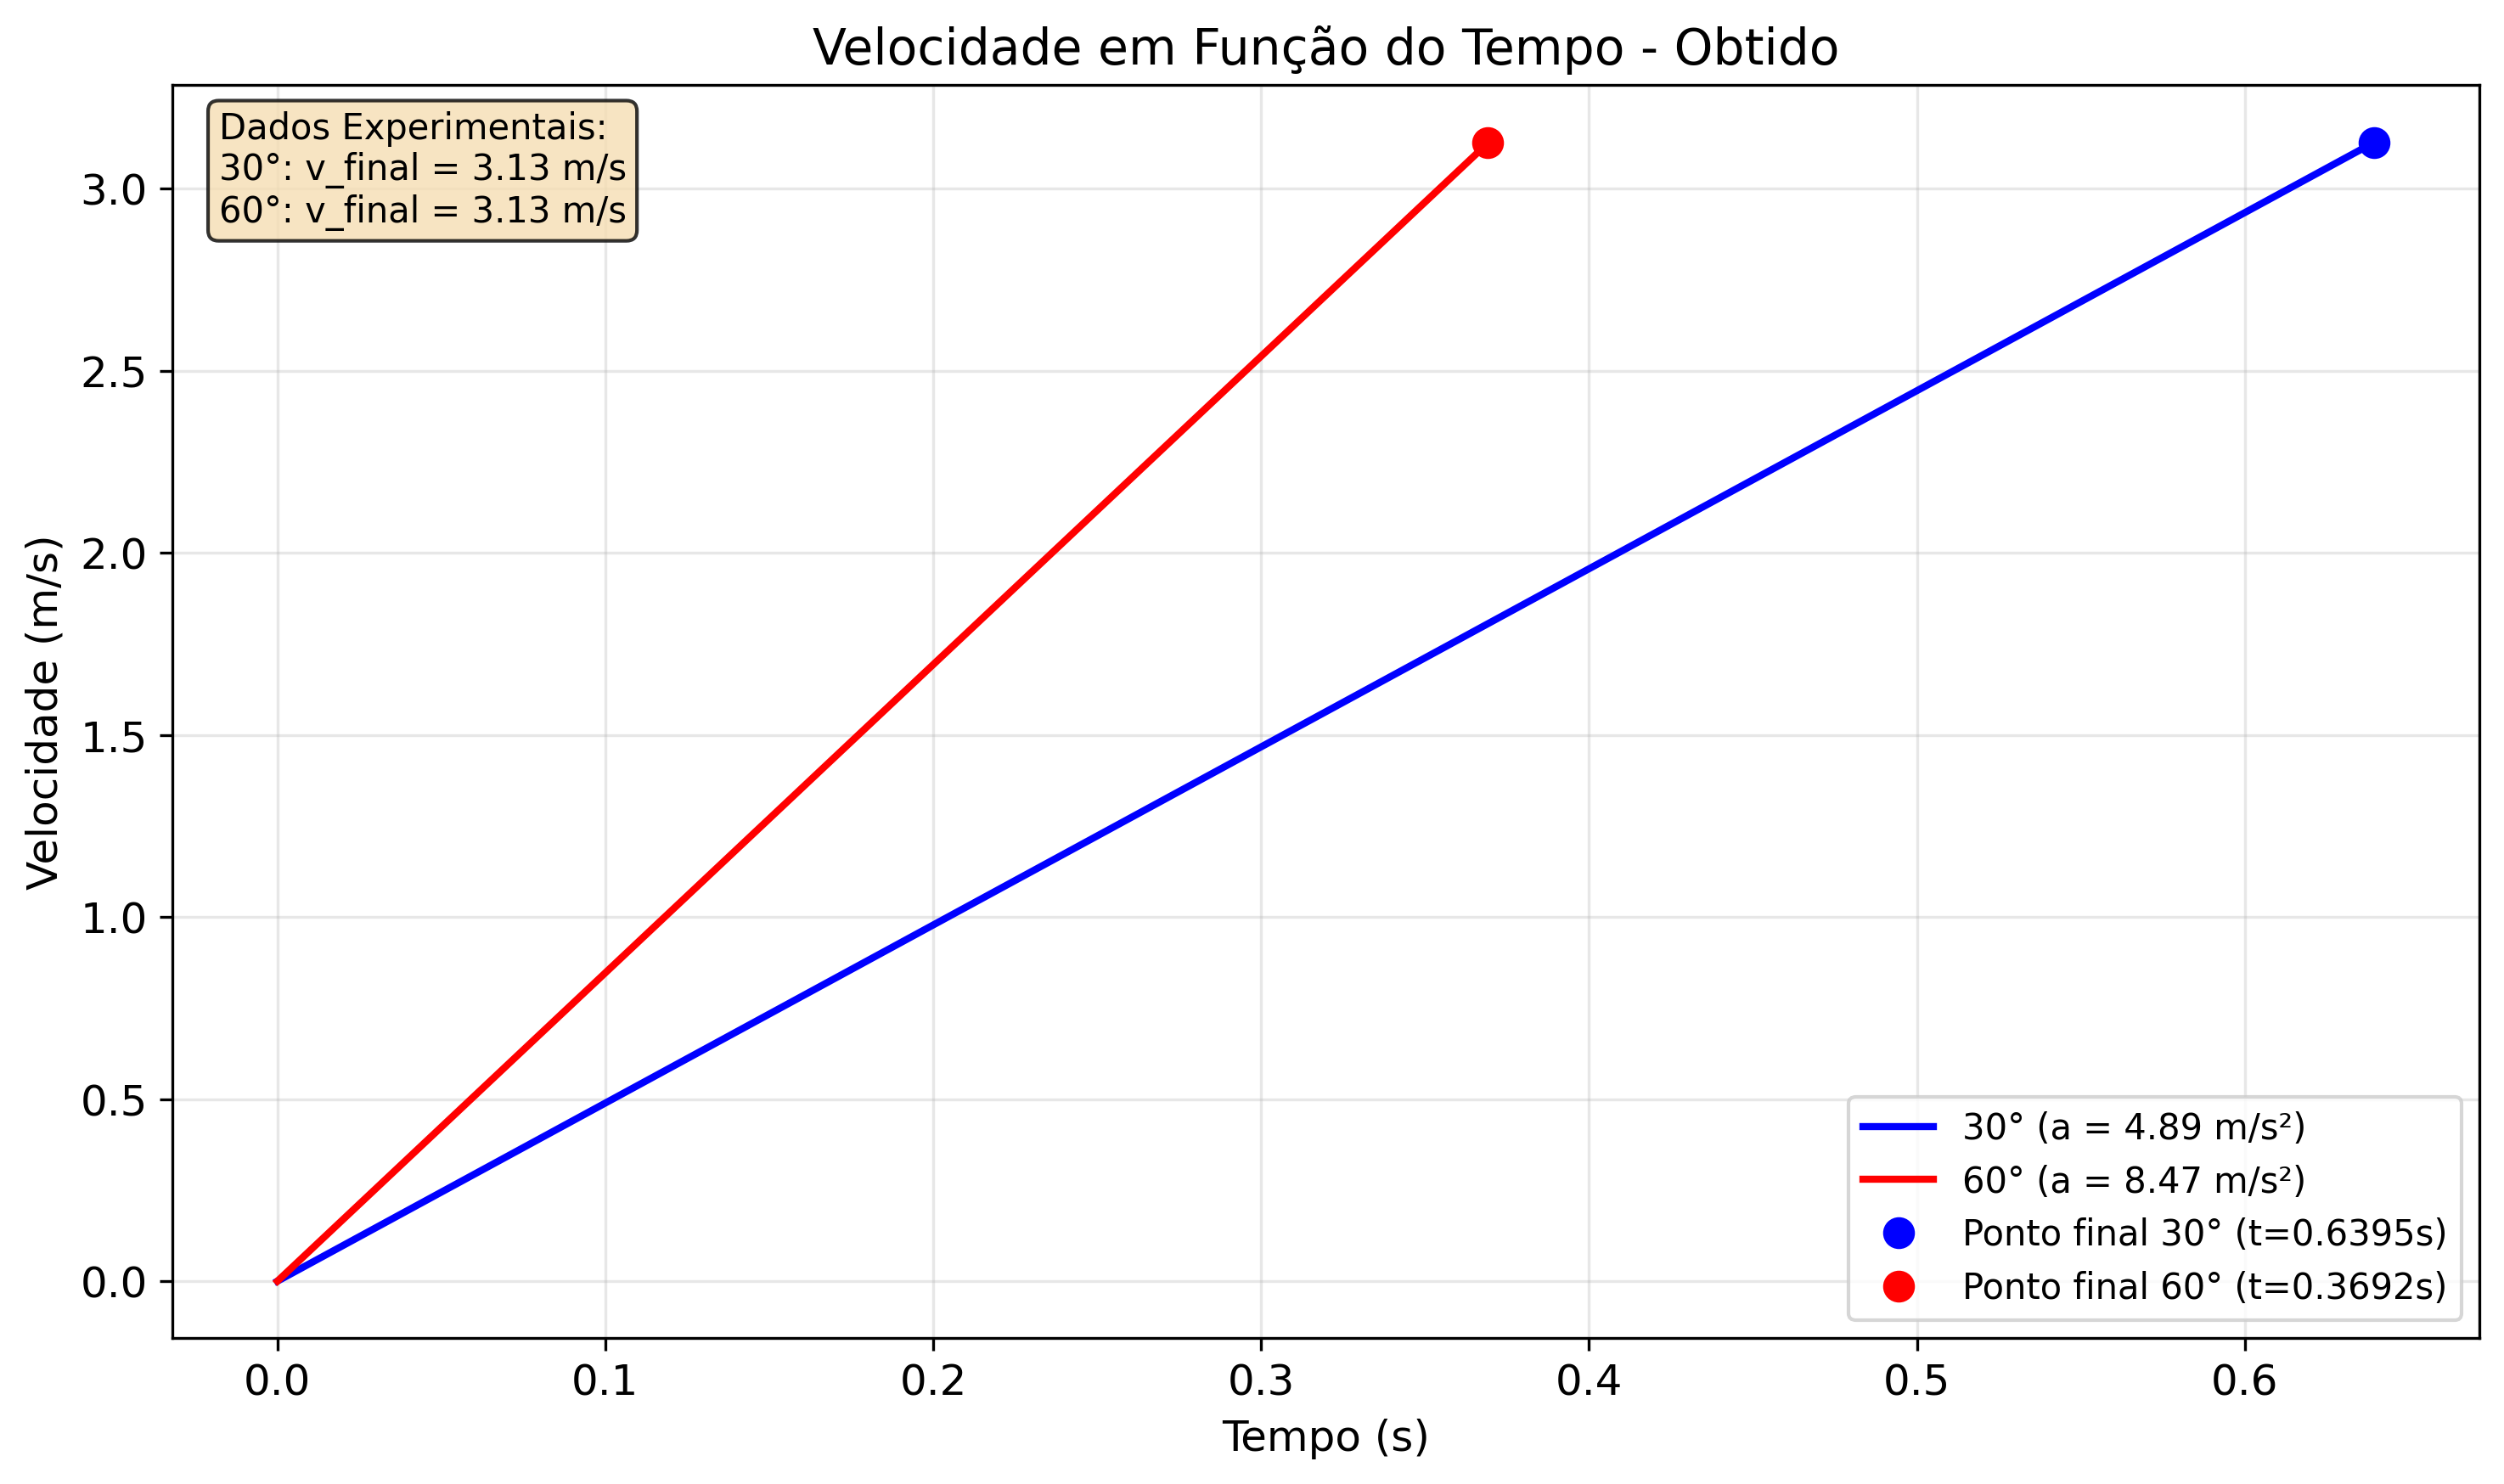
\includegraphics[scale=0.3]{./pictures/velocidade_tempo_esperado.png}
	\label{fig:velocidade_tempo_esperado}
	Fonte: Elaborado pelos autores utilizando Python (Matplotlib e NumPy).
\end{figure}
\section{Conclusão}
O experimento de determinação da aceleração da gravidade através do plano inclinado de Galileu foi realizado com sucesso, permitindo a obtenção de um valor experimental de $g = 8,06$ m/s².

Embora o erro relativo de 17,9\% em relação ao valor teórico seja significativo, este resultado está dentro do esperado para experimentos realizados com instrumentação simples e medições manuais. A metodologia de Galileu demonstrou ser eficaz para a época, considerando as limitações tecnológicas do século XVII.

O experimento validou os princípios fundamentais do movimento uniformemente acelerado e confirmou que a aceleração em um plano inclinado é proporcional ao seno do ângulo de inclinação. A consistência entre os resultados obtidos nos dois ângulos diferentes (30° e 60°) reforça a validade da abordagem experimental.

Este trabalho evidencia a importância histórica dos experimentos de Galileu para o desenvolvimento da física moderna e demonstra como princípios fundamentais podem ser investigados através de experimentos relativamente simples, os quais são de suma relevância para a compreensão de prática e teórica dos princípios fundamentais da física clássica. Atuando como ferramenta educacional indispensável.

%\onecolumn

\bibliographystyle{unsrt}
\bibliography{biblio.bib}

\end{document}